\documentclass[11pt, a4paper, twocolumn]{article}
\usepackage[utf8]{inputenc}
\usepackage{multicol}
\usepackage{fancyhdr}
\usepackage{setspace}
\usepackage{indentfirst}
\usepackage{amsmath}
\usepackage{graphicx}
\usepackage{caption}
\captionsetup[table]{singlelinecheck=false}
\usepackage[subrefformat=parens,labelformat=parens]{subcaption}
\usepackage[a4paper]{geometry}
\geometry{top=1.95cm, bottom=1.8cm, left=2.4cm, right=2.4cm, headsep=0.5cm, headheight=1cm, 
            footskip=0in, footnotesep=0in, marginparwidth = 0pt,
            hoffset=0in, voffset=0cm}
\setlength{\parskip}{0cm}
\renewcommand{\baselinestretch}{1} 
\usepackage{hyperref}
\usepackage[backend=bibtex,style=numeric-comp,sorting=none,firstinits=true,maxbibnames=99]{biblatex}
\DeclareNameAlias{author}{last-first}
\bibliography{reference}


\pagestyle{fancy}
\renewcommand{\headrulewidth}{0pt}
\fancyhf{}
\rfoot{\thepage}

\usepackage{sectsty} 
\sectionfont{\fontsize{12}{15}\selectfont}
\subsectionfont{\fontsize{12}{15}\selectfont}


\usepackage{lipsum}  

\makeatletter
\renewcommand{\maketitle}{\bgroup\setlength{\parindent}{0pt}
\begin{flushleft}
  \onehalfspacing
  \fontsize{20}{23}\selectfont
  \textbf{\@title} \\
  \hfill \break
  \fontsize{12}{15}\selectfont
  \@author
\end{flushleft}\egroup
}
\makeatother

\title{Data Retrieval via \\Natural Language Processing}
\author{%
        \textbf{Marie Cho,  Changxu Liu}\\
        \fontsize{11}{14}\selectfont
        Insitute for Computing in Research\\
        August 4th, 2022
        }

\begin{document}

\twocolumn[
  \begin{@twocolumnfalse}
    \maketitle

\noindent \textbf{Abstract.} Modern devices allow users to search for certain files, but solely utilize the names of the files, instead of the contents stored within. As humanity progresses technologically, the increasing amounts of data will serve as a barrier to a practical application of the latter task in terms of time and cost. This will necessitate accurate methods for finding information in a timely and effective manner. In this work, we create a system to search for relevant content within texts and images in respect to a user’s queries utilizing NLP that is both productive and accurate when tested on over 300,000 sources of data. \\

\noindent \textbf{Keywords:}  Deep learning, natural language processing, neural networks

  \end{@twocolumnfalse}
  \vspace{1.5em}
]

% \begin{multicols}{2}

\section{\Large{Introduction}}
Data retrieval systems using deep learning have advanced drastically and been a popular and heavily researched topic for the past several years. Latest developments in natural language processing (NLP) allow  incorporating contexts and complex lexical structures into data representations or embeddings, which in turn enables contextual understanding in the model.

While many modern devices now implement software to search for file names on the computer, most do not allow searches for the content within files themselves. The nature of the latter is restricted by techniques used with mass files and broad domains. Recent models attempting to successfully achieve this task are based on word frequencies and statistics rather than the semantics of the text.

\section{\Large{Background}}
\subsection{Natural Language Processing}
Natural Language Processing (NLP) is concerned with the ability for computers to understand human speech and text. The field of NLP began with hopes for an automatic translator after realizing the importance of interlingual communication. Today, NLP is used in translators, grammar and spell check, and virtual assistants. 

\subsection{Neural Networks}
\subsubsection{Recurrent Neural Networks}
Recurrent neural networks are commonly used in tasks concerning sequential data, such as that which is found in natural language processing. These are neural networks that contain a short term memory by being able to factor in the result of a previous element of a sequence into the processing of the next. 

\begin{figure}[htp]
    \centering
    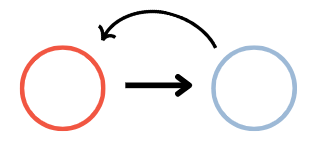
\includegraphics[width=4cm]{rnn.png}
    \caption{Recurrent Neural Networks}
    \label{fig:rnn}
\end{figure}

\subsubsection{Convolutional Neural Networks}
When dealing with visual data, convolutional neural networks are frequently used to extract their features. Convolutional neural networks function by passing filters, called kernels, through an input. These kernels represent various features that may be present in the data, such as an edge or basic geometric shape. By performing matrix multiplication, activation values are created to represent how well different sections of an image match up with the kernel, and the feature it represents. The results may be passed through multiple layers to find increasingly sophisticated features.

\begin{figure}[htp]
    \centering
    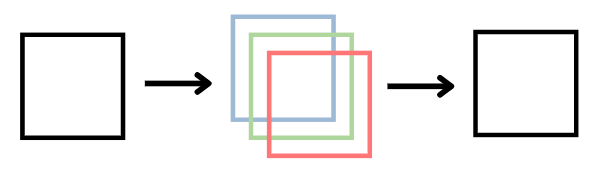
\includegraphics[width=6cm]{cnn.png}
    \caption{Convolutional Neural Networks}
    \label{fig:cnn}
\end{figure}

\subsubsection{Computer Vision}
Computer vision (CV) is concerned with the ability for computers to understand and process visual data. The field of computer vision started with the detection of basic edges and geometric shapes.  Applications of this technology include self driving vehicles, facial recognition, and optical character recognition. 

\subsection{Transformers and the BERT Model}
A transformer model is a neural network that adopts self-attention, the ability to weigh the significance of a part of data. Transformers are primarily used in NLP and CV. One transformer model highlighted in this project is the Bidirectional Encoder Representations from Transformers (BERT) Model, an unsupervised machine learning algorithm by Hugging Face to allow computers to understand the meanings of specific text and convert human language into semantic embeddings, or vectors.

\subsection{K-Means Clustering}
K-Means Clustering is an unsupervised machine learning algorithm for vector organization by which all the vectors in a space is separated into {k} groups. In this process, it will form {k} random centroids and will assign each vector to the closest centroid, labeled 1, 2, 3 ... {k}. Through trial and error, centroids will adjust themselves by taking the average of the vectors in its each respective cluster. This process is repeated over multiple iterations until in two consecutive runs, the centroids do not move or the adjustment is minimal. 

\section{\Large{Data Processing}}
\subsection{ PDF Text Extraction} 
For most PDFs, the PyPDF2 Python module was used to extract printed text data. 

However, in other cases, PDF files may be scanned documents, in which there will only be image data present in the document, which is not searchable. In order to extract the text data within, optical character recognition (OCR) is used. 

Initially, we used the Pytesseract OCR module to effectively pull printed text data out of an image. However, it was unable to properly read handwritten text data accurately with the vast amount of variation present.

A separate system was implemented to convert handwritten text into a retrievable format. To be able to properly extract handwritten text data, the handwritten text must first be located and isolated within each page before being fed into the model. Our method involved utilizing transforms in the OpenCV library to highlight text contours in scanned data. 

\begin{figure}[htp]
    \centering
    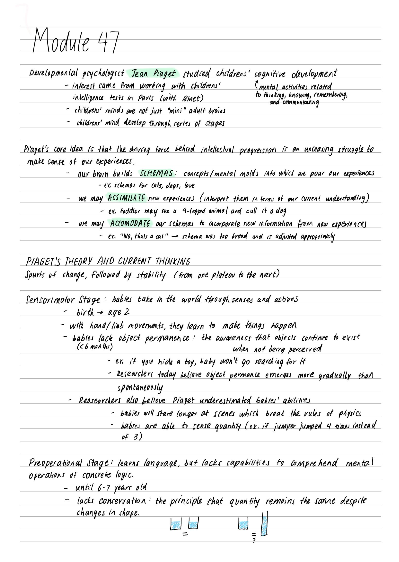
\includegraphics[width=5.3cm]{5.png}
    \caption{Handwriting document to preform OCR on.}
    \label{fig:cnn}
\end{figure}

\begin{enumerate}
\item  The scanned image is converted to grayscale and its colors are inverted. 
\item  A threshold is applied to convert each pixel to either 0 or its max value. This helps improve the contrast, makes the lighting consistent, and reduces any noise.
\item  The remaining contours on the image are dilated in the x direction to consolidate each line of text into one shape.
\item  The coordinates of a rectangular bounding box are recorded and used to crop out each individual line. 
\end{enumerate}

\begin{figure}[htp]
    \centering
    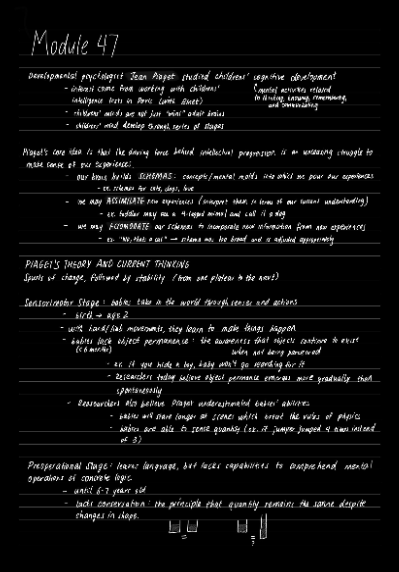
\includegraphics[width=3.5cm]{1.png}
    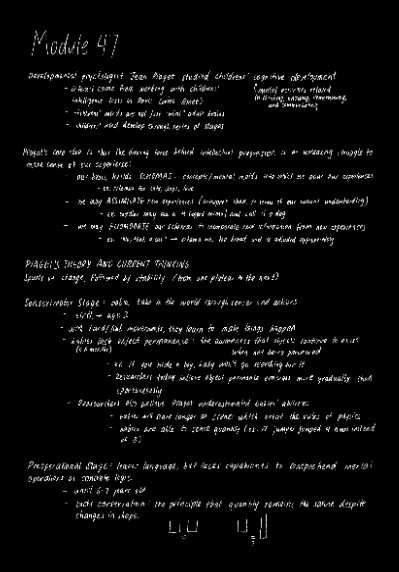
\includegraphics[width=3.5cm]{2.png}
    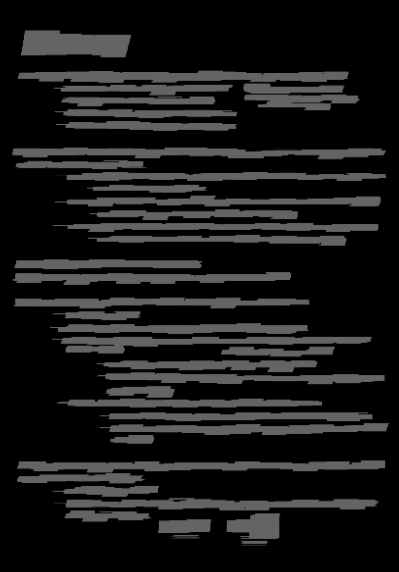
\includegraphics[width=3.5cm]{3.png}
    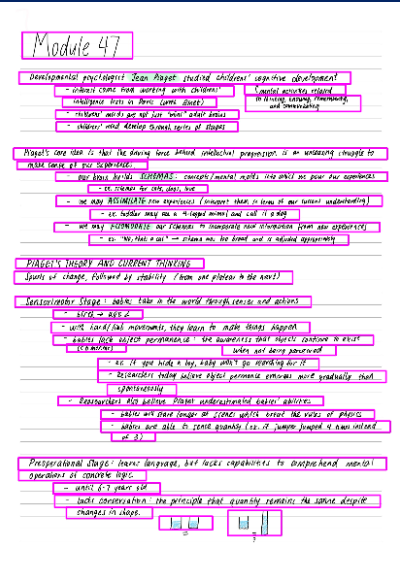
\includegraphics[width=3.5cm]{4.png}
    \caption{OCR}
    \label{fig:cnn}
\end{figure}

This method presents limitations to the format of image data in which text may be detectable. However since our main focus is on scanned documents for data retrieval, this should be adequate. Then, with each line of text cropped, it can be fed into a convolutional neural network to perform feature extraction. Afterwards, the resulting feature map can be put into a recurrent neural network to propagate relevant features. Finally, we can use Connectionist Temporal Classification (CTC) to decode our data into text.

\subsection{Image Captioning} 
For pure images and photographs that don’t contain any text, generating a caption to describe the image will need to be done to make it searchable. To do this, a convolutional neural network is utilized to extract features from the input image. We used the pre-trained 50 layer variant of the deep ResNet model. Unique for its residuals which pass data through certain layers, it helped reduce the degradation problem, where the accuracy of neural networks decreased with a greater number of layers. 

Because classification isn’t needed, the final fully-connected layer is removed from the network, and the features are then passed into a recurrent neural network, which decodes the feature vector into a basic caption that can be used to describe the image. 

This model was trained on the Flickr8K dataset, which we believed would represent photos an individual may need to search through on a computer.

\begin{figure}[htp]
    \centering
    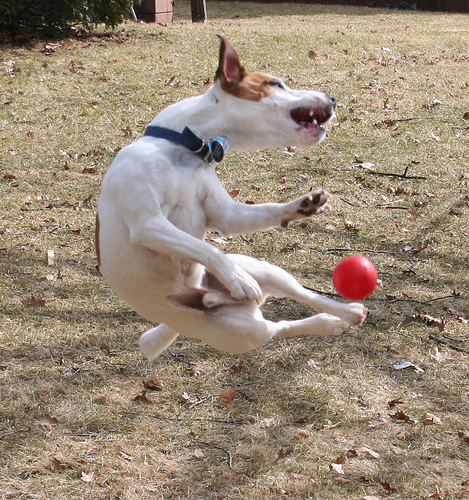
\includegraphics[width=4.5cm]{128912885_8350d277a4.jpg}
    \caption{"a white dog is jumping up to catch a ball in a field."}
    \label{fig:cnn}
\end{figure}

\begin{figure}[htp]
    \centering
    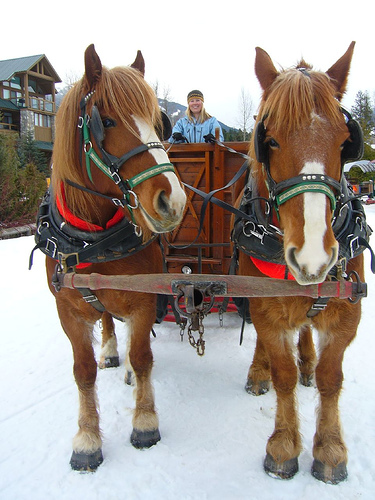
\includegraphics[width=4.5cm]{109202801_c6381eef15.jpg}
    \caption{"two horses pull a carriage driven by a man in a blue jacket. "}
    \label{fig:cnn}
\end{figure}

\section{\Large{Data Retrieval}}

\subsection{The BERT Model} 
Within the vast field of NLP are various language models that have been developed to make such innovations possible. The BERT Model, an unsupervised machine learning algorithm, allows computers to understand the meanings of specific text. This serves as the bridge between human language and semantic embeddings, allowing the text files and queries to be comparable numerically. When a text is inputted into BERT, the model will create a tensor vector with numerical values equivalent to the meaning of the text.
\subsection{Determining Proximity} 
Two important methods of measuring the similarity between vectors in space are the Cosine Similarity and the Euclidean Distance. Although each has their own advantages, they take different approaches of determining proximity.
\subsubsection{Cosine Similarity}
Cosine Similarity is a measure of proximity between two vectors by determining the cosine of the angle between them. Thus, the smaller the angle difference, the higher the similarity score. Two vectors of equal orientation (0°) have a maximum similarity of 1, two vectors that are orthogonal (90°) have a similarity of 0, and two vectors that lie directly opposed to each other (180°) have a minimum similarity of -1. This method is therefore a judgement of orientation and direction, independent of the vectors' magnitude and weight. 
\begin{align} 
\label{cos}
cos(A,B) &= \frac{A\cdot B}{\|A\| \|B\|}\nonumber
\end{align}
\subsubsection{Euclidean Distance}
In contrast, Euclidean Distance is the distance between two points in space, or the length of a line segment connecting those two points. Thus, this method does consider a vector's magnitude and weight when calculating the proximity.
\begin{align} 
\label{eu}
d(A, B) &= \sqrt{(x_2-x_1)^2 + (y_2-y_1)^2}\nonumber
\end{align}
Rather than finding the physical distance between two points,  finding the angle measure between vectors is more accurate when using NLP. Because texts can vary in terms of size and length yet can contain the same meaning as another, thus the same orientation, cosine similarity is more effective in catching the semantics and therefore more practical in this scenario.
\begin{figure}[htp]
    \centering
    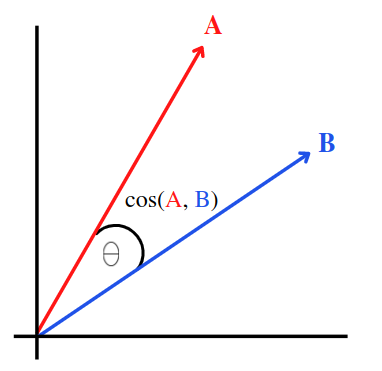
\includegraphics[width=3cm]{cos_sim.png}
    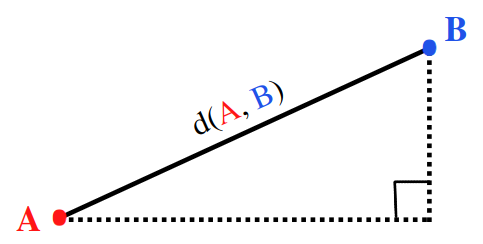
\includegraphics[width=4cm]{eu_dist.png}
    \caption{Cosine Similarity vs Euclidean Distance}
    \label{fig:cos_vs_eu}
\end{figure}
\subsection{Acceleration through K-Means Clustering} 
In preparation for the experiment, we used normalized the vectors using L2 normalization. Two different modes are used: base (without optimization) and kmeans (with optimization using k-means clustering and reference vectors). All loading and query times are recorded for numerical representations of each reference point's efficiency.

Finding the most relevant item in terms of cosine similarity is equivalent to finding the one with the lowest Euclidean distance. To speed up the top-k nearest neighbor search, it is critical to reduce the number of cosine similarity computations between a query and the items. Hence, we can limit our search to the cluster with the minimum distance between a query and the centroid.

When k=1, it degenerates to a full-blown search. When $k > 1,$ it will reduce the overall search time but with the risk of sub-optimal search results. For example, when the embedding vector of a query is on the boundary between two clusters, our acceleration scheme focuses on the one with the closer distance, hence leaving out some high-quality items from the search. The larger the k for clustering, the higher the chance of sub-optimal results but the lower the wait time.

\section{\Large{Results}}

\subsection{Base}
The base mode took around 17 seconds to load and prepare and about 7 seconds to calculate the top 5 nearest neighbor vectors for each of the 10 queries. While the base mode is the 100\% accurate since it compares the query to every sentence in the text documents, times will get increasingly slower as the system is exposed to more and more data.

\begin{figure}[htp]
    \centering
    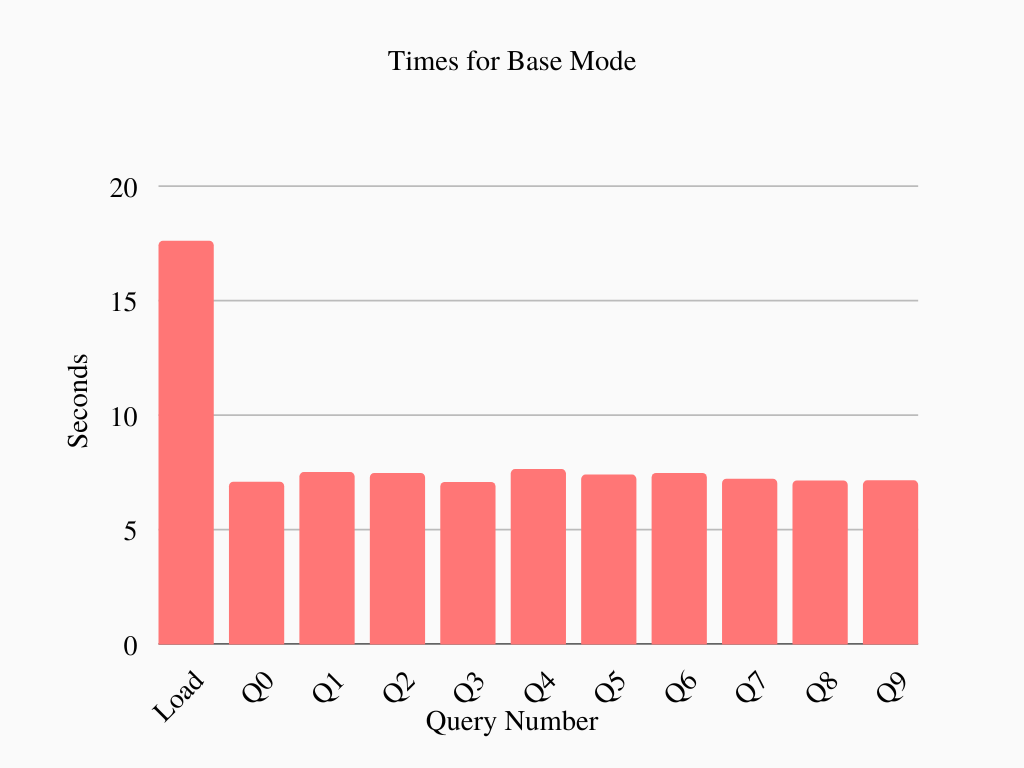
\includegraphics[width=7cm]{base.png}
    \caption{Loading and Query Times for Base Mode}
    \label{fig:base}
\end{figure}
\subsection{{K}-Means Clustering}
We experimented with 6 runs using various k values in the kmeans mode. As shown in the graph, query times have decreased as the number of centroids increased. Ideally, at some point the time will be essentially 0 seconds. However, there is a constant factor present that cannot be optimized, so there will always be some amount of wait time. Despite this, the overall wait time has reduced significantly.

\begin{figure}[htp]
    \centering
    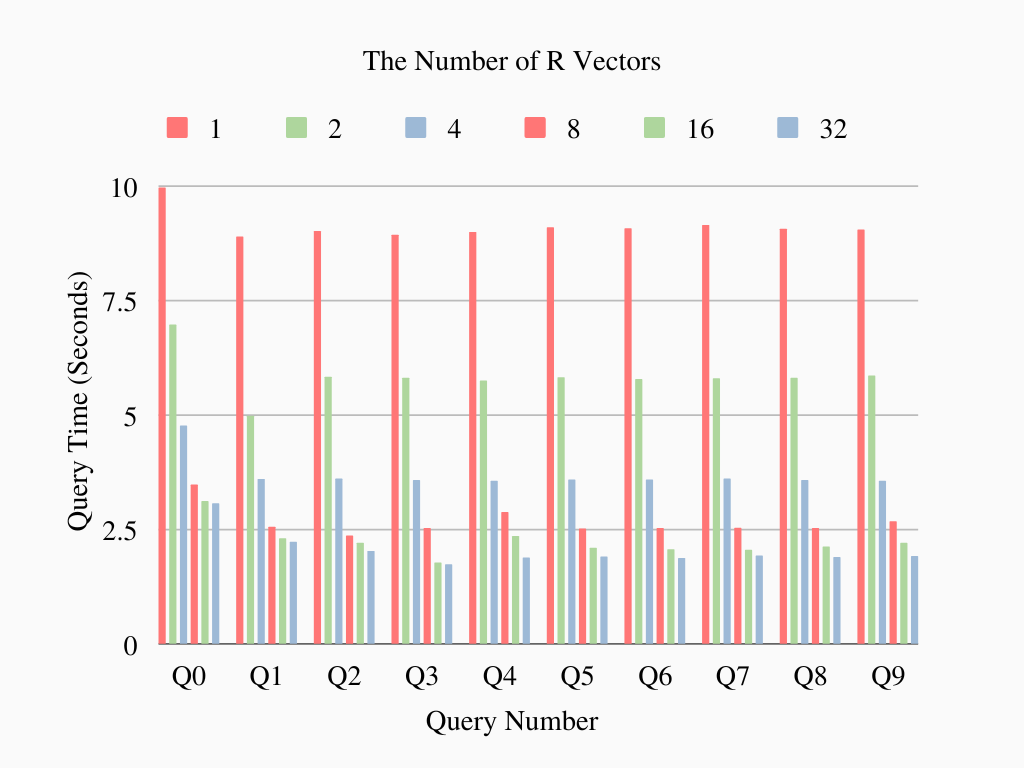
\includegraphics[width=7cm]{kmeans_query.png}
     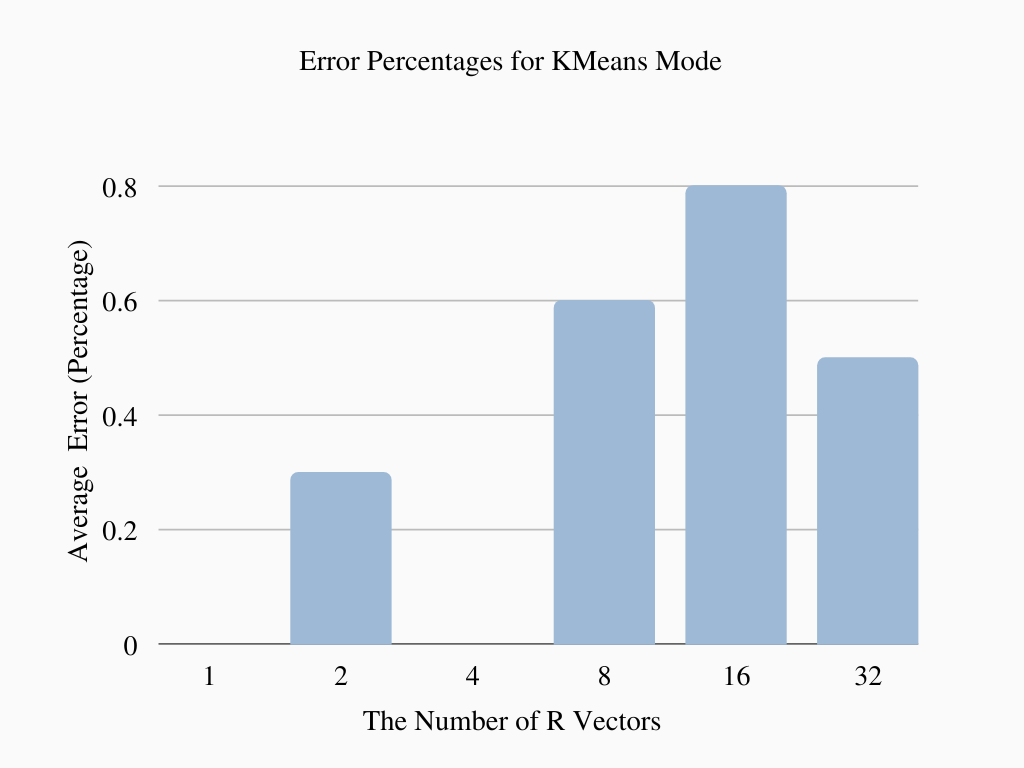
\includegraphics[width=7cm]{kmeans_err.png}
    \caption{Query Times and Error Percentages for K-Means Mode}
    \label{fig:kmeans}
\end{figure}
This comes as a trade-off with a risk of errors and inaccuracy. However, because errors occur by chance, the accuracy of the search result can waver. Although overall errors increase, the average percentages remain less than 1\%. Note that both factors may go above these thresholds as {k} increases above 32.

\section{\Large{Future Work}}
Throughout this project, we have been able to produce a data retrieval system through the use of natural language processing in addition to machine learning and neural networks. While our program has been optimized and improved, we believe that further steps could be taken in the future to make this project more advanced. These are multiple next steps that can be taken to build on these findings:
\begin{enumerate}
\item Optimizing memory usage for the ability to search and sort through a even larger mass of files
\item Improving the accuracy of search results 
\item Generating more detailed image captions
\item Better format recognition in OCR 
\end{enumerate}
\section*{Acknowledgements}
We would like to sincerely thank Optiver for providing us their space during this internship, Mark Galassi and Rhonda Crespo for running the ICR and giving us this research opportunity, our fellow interns and Mark Emry for being supportive along the way, and finally our mentor Jim Davies for guiding us through this project.

\begin{thebibliography}{30}
\bibitem{article}
Rebecca Reynoso (2021) \emph{A Complete History of Artificial Intelligence}, G2.

\bibitem{article}
Shamala Gallagher, Anna Rafferty, and Amy Wu (2004) \emph{Natural Language Processing}, Stanford University.

\bibitem{article}
Rani Horev (2018) \emph{BERT Explained: State of the art language model for NLP}, Towards Data Science.

\bibitem{article}
Daniela M. Witten and Robert Tibshiran (2010) \emph{A Framework for Feature Selection in Clustering}, Journal of the American Statistical Association.

\bibitem{article}
Nandan Thakur, Nils Reimers, Johannes Daxenberger, and Iryna Gurevych (2021) \emph{Augmented {SBERT}: Data Augmentation Method for Improving Bi-Encoders for Pairwise Sentence Scoring Tasks}, Proceedings of the Conference of the North American Chapter of the Association for Computational Linguistics.

\bibitem{article}
Jacob Devlin, Ming-Wei Chang, Kenton Lee, Kristina Toutanova (2018) \emph{BERT: Pre-training of Deep Bidirectional Transformers for Language Understanding}, arXiv

\bibitem{article}
Fabian Pedregosa, Gaël Varoquaux, Alexandre Gramfort, Vincent Michel, Bertrand Thirion, Olivier Grisel, Mathieu Blondel, Peter Prettenhofer, Ron Weiss, Vincent Dubourg, Jake Vanderplas, Alexandre Passos, David Cournapeau, Matthieu Brucher, Matthieu Perrot, Édouard Duchesnay (2011) \emph{Scikit-learn: Machine Learning in Python}, JMLR

\bibitem{article}
Paszke et al (2019) \emph{PyTorch: An Imperative Style, High-Performance Deep Learning Libary}, Curran Associates Inc.

\bibitem{article}
C.R. Harris, K.J. Millman, S.J. et al. van der Walt (2020) \emph{Array programming with NumPy}, Nature

\bibitem{article}
Kaiming He, Xiangyu Zhuang, Shaoqing Ren, Jian Sun (2015) \emph{Deep Residual Learning for Image Recognition}, arXiv

\bibitem{article}
Micah Hodosh, Peter Young, Julia Hockenmaier (2013) \emph{Flickr8K Dataset}, Journal of Artificial Intelligence Research

\bibitem{article}
Ray Smith (2007) \emph{An Overview of the Tesseract OCR Engine}, IEEE

\bibitem{article}
Ralf C. Staudemeyer (2019) \emph{Understanding LSTM -- a tutorial into Long Short-Term Memory Recurrent Neural Networks}, arXiv

\bibitem{article}
Bradski, G. (2000) \emph{The OpenCV Library}, Dr. Dobb's Journal of Software Tools

\end{thebibliography}

\end{document}

